\documentclass[a4paper,10pt,twocolumn]{article}
\title{\textbf{\underline{REPORT: Logistic Regression}}}
\usepackage[left=2cm, right=2cm, top=1.5cm]{geometry}
\usepackage{xcolor}
\usepackage{ragged2e}
\usepackage{lipsum,multicol}
\usepackage{hyperref}
\usepackage{graphicx}
\usepackage{subfig}
\usepackage{amsmath, amsfonts}
\usepackage{times}
\date{}
\author{}
\begin{document}
\maketitle
%===================================================================================================================%
\section*{\textcolor{blue}{1. Introduction:}}
In this report, we try to analyse the performance (accuracy, fscore, recall and precision) of a logistic regression that we built using NumPy. The implementation of this network is similar to that of sklearn and the whole code has been written in a completely modularized fashion.

\section*{\textcolor{blue}{2. Data Preprocessing:}}
The dataset contained 1372 data points, each containing 4 input features (representing banknote features) and one binary target variable (representing if the note is authentic or not). In the preprocessing stage, all features were standardized and randomly split into \textit{train\_set}, \textit{test\_set} and \textit{validation\_set}  (70-20-10 split ratio).

\section*{\textcolor{blue}{3. Non-Linear function:}}
\begin{itemize}
\item{sigmoid: $y$ = $\frac{1}{1 + e^{-x}}$}
\end{itemize}

\section*{\textcolor{blue}{4. Loss function:}}
\begin{itemize}
\item{$L_n = \sum_{n=0}^{N} -t_nlog(y_n)-(1-t_n)log(1-y_n)$} 
\end{itemize}

\section*{\textcolor{blue}{5. Model Architecture:}}
\subsection*{\textcolor{red}{5.1 Vanilla Logistic Regression:}}
The architecture of our model resembles that of a single layer perceptron. The predictions for the whole training set were made according to the following formula: $\sigma(\widetilde{W}^T \widetilde{X})$ where $\widetilde{X}$ represents the input features padded with ones to accomodate the bias term and $\sigma$ represents the sigmoid function. The Log Loss function mentioned above is a strictly convex function in the case of logistic regression and hence, only one global minima will exist. Any initiliazation of weights must converge at the global minima. \textit{Gradient Descent} was used as the optimizing function in this case, i.e. the gradient with respect all training points was considered in order to make the ``down hill step".
\newline
\newline
\underline{Top metrics achieved by the model:}
\begin{itemize}
\item{Best testing accuracy: $99.64\%$}
\item{Best testing recall: $99.28\%$}
\item{Best testing precision: $100.0\%$}
\item{Best testing fscore: $99.64\%$}
\end{itemize}
These metrics were achieved with 15000 epochs and a \textit{learning\_rate} of 0.01. In this case, we don't observe much difference in the 

\subsection*{\textcolor{red}{5.2 Logistic Regression with L1 regularization:}}
Regularization in Regression/Neural Network helps curb over-fitting. When given no restriction on the weights, the parameters can verly likely assume high values and overfit the training data. So, to control these weights from growing abnormally large, we introduce regularization. In L1 regularization, an additional term of $\frac{\lambda}{2}$ $|W|$ is added to the loss function where $\lambda$ is the regularization hyperparameter. In our model, the value of $\lambda$ was searched between 0.0 and 1.5, and the value which gave the highest accuracy (or any metric, which could be explicitly specified) on the validation data, was chosen as the optimal L1 hyperparameter.
\newline
\newline
\underline{Top metrics achieved by the model:}
\begin{itemize}
\item{Best testing accuracy: $98.18\%$}
\item{Best testing recall: $100.0\%$}
\item{Best testing precision: $95.68\%$}
\item{Best testing fscore: $97.79\%$}
\end{itemize}
These metrics were achieved with 15000 epochs and a \textit{learning\_rate} of 0.01. In our case, not much difference in accuracy was observed even when L1 regularization was implemented. But the weights obtained initially were a bit a large and weights were slightly reduced due to the constraint.
\textbf{Optimal lambda:} 0.107

\subsection*{\textcolor{red}{5.3 Logistic Regression with L2 regularization:}}
This technique is the most popular regularization method and similar to L1 regularization. In this case, an extra term of $\frac{\lambda}{2}$ $|W|^2$ is added to the loss function in order to curb higher weights and overfitting. Once again, the value of $\lambda$ was searched between 0.0 and 1.5, and the value which gave the highest accuracy (or any metric, which could be explicitly specified) on the validation data, was chosen as the optimal L2 hyperparameter.
\newline
\newline
\underline{Top metrics achieved by the model:}
\begin{itemize}
\item{Best testing accuracy: $98.18\%$}
\item{Best testing recall: $100.0\%$}
\item{Best testing precision: $95.68\%$}
\item{Best testing fscore: $97.79\%$}
\end{itemize}
These metrics were achieved with 15000 epochs and a \textit{learning\_rate} of 0.01. In our case, not much difference was in accuracy was observed even when L2 regularization was implemented (values obtained were very similar to that of L1 regularization). But the weights obtained initially were a bit a large and weights were reduced due to the constraint.
\textbf{Optimal lambda:} 0.107

\section*{\textcolor{blue}{6. Feature Importance:}}
One of the simplest options to get a feeling for the "influence" of a given parameter in a linear classification model (logistic being one of those), is to consider the magnitude of its coefficient times the standard deviation of the corresponding parameter in the data. Since our data is standardized, we just need to consider the magnitude of the weight. The weights (absolute values) obtained were: [$10.97247675$, $22.50767307$, $25.61193349$, $23.30568063$, $1.4515536$], where the first term denotes the bias. The largest coefficient is that of the second feature and the feature of least importance is fourth feature. Ranking the features by their importance, i.e. their magnitudes: [$2, 3, 1$, bias, $4$]. Now if we look at the original weights then a negative coefficient means that higher value of the corresponding feature pushes the classification more towards the negative class. 
\href{https://stackoverflow.com/questions/51462979/how-to-get-feature-importance-in-logistic-regression-using-weights}{[Ref-1]}
\href{https://stackoverflow.com/questions/34052115/how-to-find-the-importance-of-the-features-for-a-logistic-regression-model}{[Ref-2]}


\section*{\textcolor{blue}{7. Conclusion:}}
\begin{itemize}
\item{The model almost everytime converged on the same point due the existence of a single global minima, and the initialization of weights didn't matter due to the same reason.}
\item{Lower learning rates give a smoother curve (as seen below) but take more number of epochs to converge. Higher learning rates aid the model to converge faster but there is always a chance that the model might just end up bouncing around the minimia and never reach it, or might even ``hop out" of the minima.}
\item{Imposing regularization didn't affect the accuracy but the weights, in the case of L2 regularization, were significantly cut down.}
\end{itemize}
[results on next page]

\newpage
\onecolumn
\section*{\textcolor{blue}{8. Results:}}
\begin{figure}[h!]
\centering
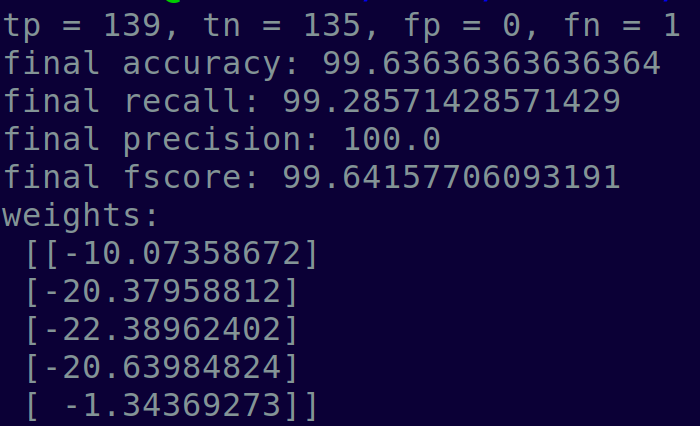
\includegraphics[scale=1.0, width=5cm]{Fig1.png}
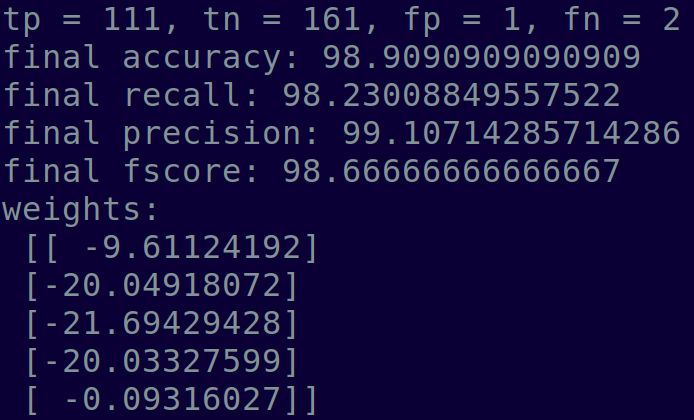
\includegraphics[scale=1.0, width=5cm]{Fig2.png}
\caption*{Logistic Regression Metrics with no regularization}
\end{figure}

\begin{figure}[h!]
\centering
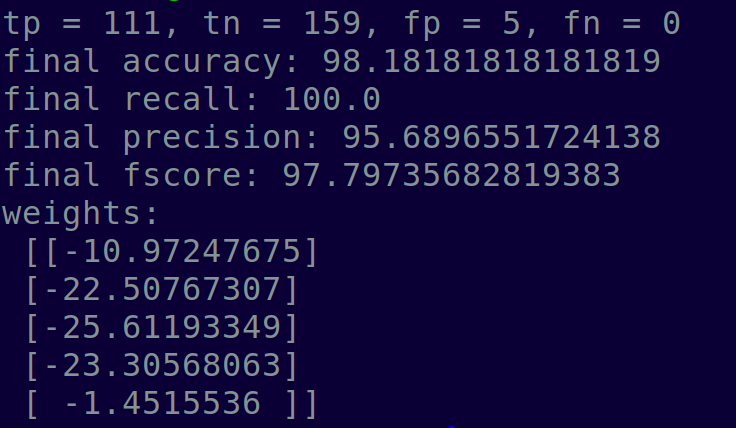
\includegraphics[scale=1.0, width=5cm]{Fig3.png}
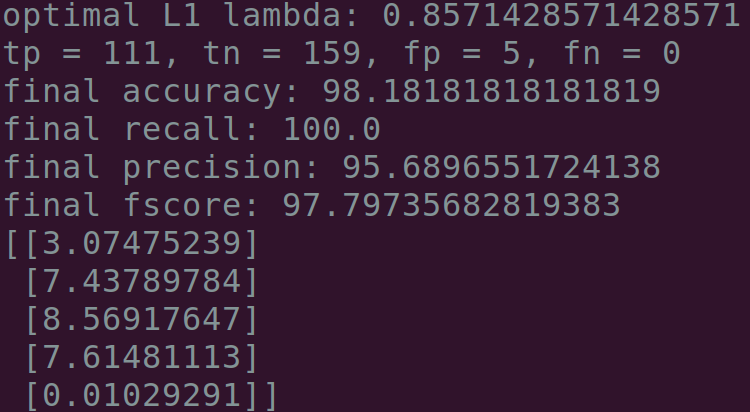
\includegraphics[scale=1.0, width=5cm]{Fig4.png}
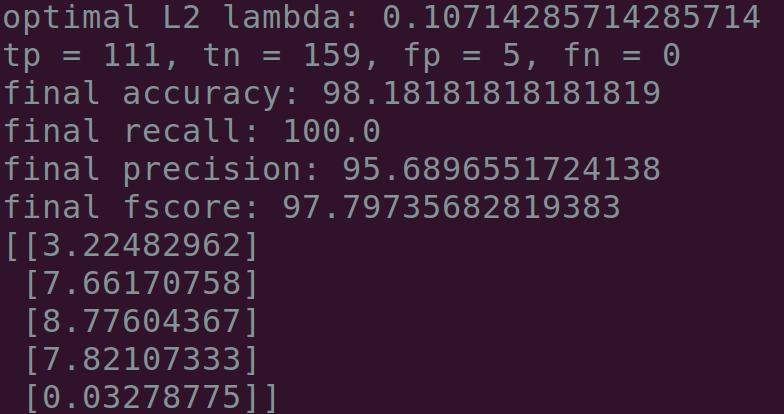
\includegraphics[scale=1.0, width=5cm]{Fig5.png}
\caption*{Logistic Regression Metrics and weights with no regularization, L1 regularization and L2 regularization wrt Accuracy}
\end{figure}

\begin{figure}[h!]
\centering
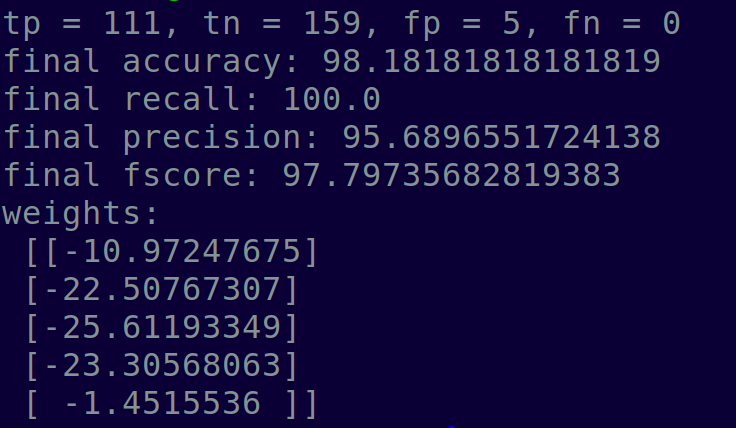
\includegraphics[scale=1.0, width=5cm]{Fig3.png}
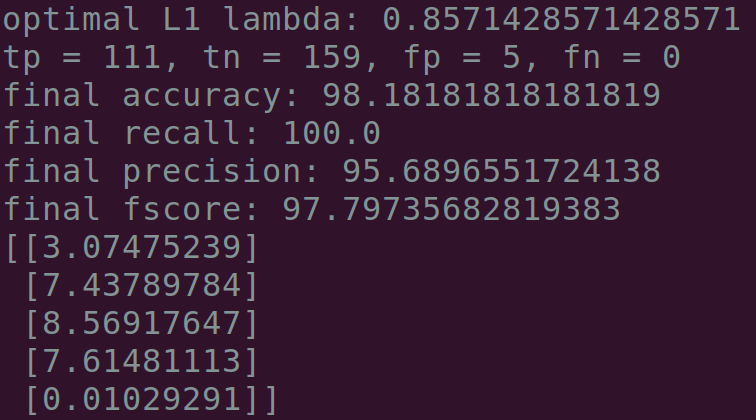
\includegraphics[scale=1.0, width=5cm]{Fig6.png}
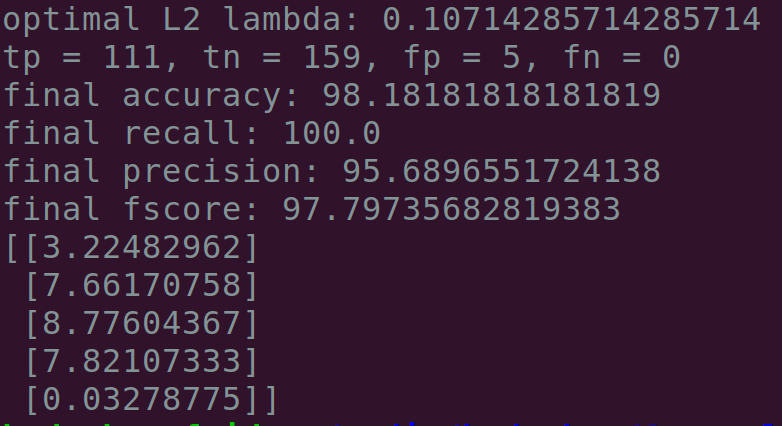
\includegraphics[scale=1.0, width=5cm]{Fig7.png}
\caption*{Logistic Regression Metrics and weights with no regularization, L1 regularization and L2 regularization wrt Fscore}
\end{figure}

\begin{figure}[h!]
\centering
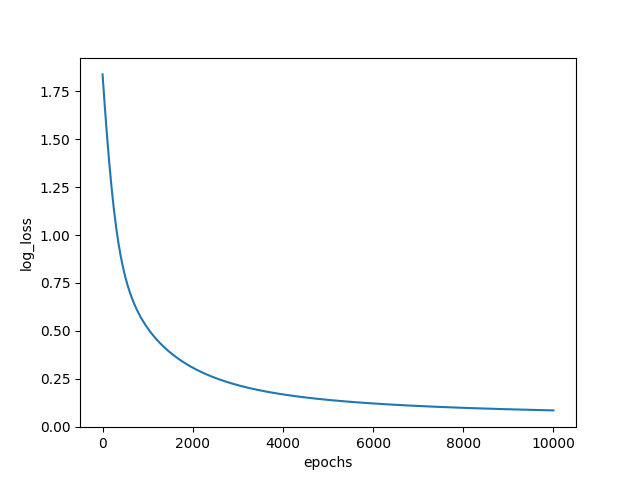
\includegraphics[scale=1.0, width=5cm]{Fig11.png}
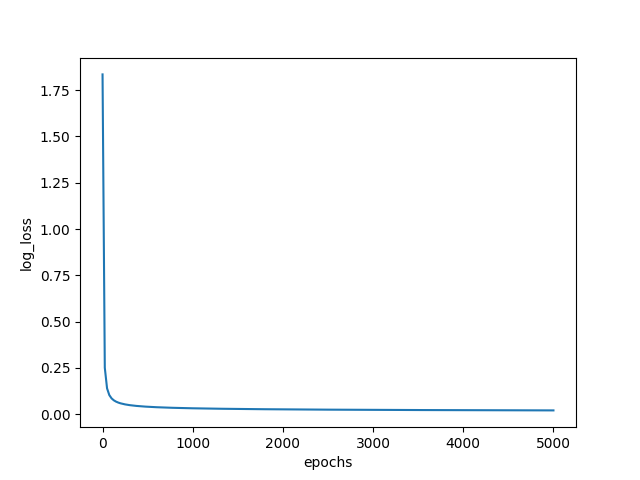
\includegraphics[scale=1.0, width=5cm]{Fig12.png}
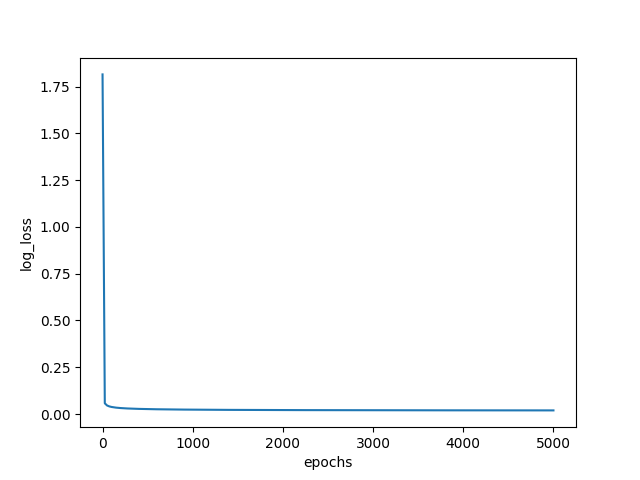
\includegraphics[scale=1.0, width=5cm]{Fig13.png}
\caption*{Loss vs Epochs for different learning rate. $(10^{-5}, 10^{-3}, 10^{-2})$. We observe that lower learning rates give smoother curves.}
\end{figure}
%=================================================================================================================%
\end{document}
